\documentclass[11pt, twoside, listof=totocnumbered, bibliography=totocnumbered]{scrartcl}

%math
\usepackage{amsmath,amssymb,amstext}

%url
\usepackage{url}

%language
\usepackage{ucs}
\usepackage[utf8x]{inputenc}
\usepackage[T1]{fontenc}
\usepackage[ngerman, main=english]{babel}
\usepackage{blindtext}

%images
\usepackage{graphicx}

%header/footer
\usepackage[
bmargin=25mm, 
tmargin=20mm,
inner=50pt,
outer=80pt
]{geometry}
\usepackage{scrlayer-scrpage}
\usepackage{lastpage}

%arrows
\usepackage{textcomp}

\usepackage{multicol}

\usepackage{hyperref}

%code listings
\usepackage{caption}
\DeclareCaptionType{code}[Codebeispiel][Codebeispielverzeichnis] 

%code (C#)
\usepackage{listings}
\usepackage{xcolor}
\definecolor{bluekeywords}{rgb}{0,0,1}
\definecolor{greencomments}{rgb}{0,0.5,0}
\definecolor{redstrings}{rgb}{0.64,0.08,0.08}
\definecolor{grey}{rgb}{0.5,0.5,0.5}
\definecolor{types}{rgb}{0.17,0.57,0.68}
\usepackage{listings}
\lstset{language=[Sharp]C,
	captionpos=b,
	numbers=left, %Nummerierung
	numberstyle=\color{grey}\scriptsize,
	frame=lines, % Oberhalb und unterhalb des Listings ist eine Linie
	showspaces=false,
	showtabs=false,
	breaklines=true,
	showstringspaces=false,
	breakatwhitespace=true,
	escapeinside={(*@}{@*)},
	commentstyle=\color{greencomments},
	morekeywords={partial, var, value, get, set},
	keywordstyle=\color{bluekeywords},
	stringstyle=\color{redstrings},
	basicstyle=\ttfamily\small,
}
%\begin{lstlisting}[caption=a test for a C$^\sharp$ code, label=lst:test]
%code
%\end{lstlisting}

%bibliography
\bibliographystyle{alpha}

%Description environment
\usepackage[strict]{changepage}
\usepackage{framed}
\definecolor{formalshade}{rgb}{0.95,0.95,1}
\definecolor{darkblue}{rgb}{0,0,0.3}
\newenvironment{desc}{%
	\def\FrameCommand{%
		\hspace{1pt}%
		{\color{darkblue}\vrule width 2pt}%
		{\color{formalshade}\vrule width 4pt}%
		\colorbox{formalshade}%
	}%
	\MakeFramed {\advance\hsize-\width \FrameRestore}}%
{\endMakeFramed}

%bsubsection
\setcounter{secnumdepth}{4}
\setcounter{tocdepth}{4}

%custom commands
\newcommand{\br}{\hfill\\}
\newcommand{\phantomtitle}[1]{\noindent\textbf{\LARGE #1 }\\\br}
\newcommand{\bt}{{\color{grey}\blindtext}}
\newcommand{\cfct}[1]{\cite{#1}}
\newcommand{\imgct}[1]{(source: \cite{#1})}
\newcommand{\bld}[1]{\textbf{#1}}

%paragraph style
\setlength{\parindent}{0pt}
\setlength{\parskip}{1em}
\title{Device for digitizing materials}
\author{Niklas Hauber}
\date{\today{}, Linz} 
\begin{document}
\maketitle
Creation date of initial version: January 2, 2023\\
Publication date of initial version: January 2, 2023\\
Modification date of current version: January 2, 2023\\

\section{Abstract}
Photometric stereo is a method to obtain information about material which describes the 3D shape of it and/or in what way it reflects light. This document is meant as a defensive publication of a product, that scans a material and calculates its 3D shape, as well as how it reflects, transmits or emits light. For example by solving the parameters of a "Spatially Varying Bidirectional Reflectance Distribution Function". The material to be scanned can be anything that reflects, emits or transmits light and can range from hot steel slabs to liquids (other examples are fabrics, leather, plants, rocks, skin, hair, photoluminescent materials and so on). The scanner uses various forms of light which differ in their form and/or spectral distribution, to illuminate the material. This is done, because combining different types of light sources will help elimite any shortcomings, which only using a single type of light would have. \cite{SURVEY}
\section{Description}
The scanner consists of the following components, many of which are optional:
\begin{enumerate}
	\item One or more cameras which image the transmission of light through or reflection of light off the material. Using multiple cameras has the advantage that more data is available for the software that processes it and a more accurate 3d representation of the object can also be calculated, by using stereophotogrammetry. The normal map calculated via the method of photometric stereo can be used in addition to the 3d model calculated by the previous step, by providing high frequency detail. One possible implementation would be adding a lowpass filtered height map optained by stereophotogreammetry and a highpass filtered height map obtained by integrating the normals obtained by photometric stereo. The cameras can either be fitted with a color filter array (CFA) or can be monochrome (optionally with a filter wheel in front), which would yield better quality images.
	\item One or more broadband point light sources (like white leds), which reflect off or transmit through the material. These are typically used by photometric stereo, as they are cheap and are easy to model mathematically. However, they are unsuitable for glossy materials with low roughness and hard shadows also cause artefacts, if not compensated for.
	\item One or more colored/spectrally variable point light sources (like colored leds/lasers or broadband light sources with filters in front of them) which reflect off / transmit through the material. Having colored light emited towards the material and filtering it after the reflection/transmission occured can be used to obtain information about photolumineszence of the material. Colored light may also be produced by controlling the angle of incidence of broadband light (for example by moving the light source or moving mirrors/lenses which reflect/refract it) to a prism (or equivalent objects like a diffraction grating, which bends or reflects the light at an angle dependent on its wavelength) and the resulting "rainbow" of light can then be mostly filtered by an opening letting only part of the light through. The resulting colored light will be rather dark (depending on the size of the opening), but one will have a rather inexpensive device that can adjust its color to any desired wavelength band.
	\item One or more linear light sources (either broadband/white or colored/spectrally variable) which reflect off the material and a camera takes a monochromatic or multispectral/colored images (with filters in front of it, either a CFA or with a filter wheel), linear light has the advantage, that it greatly improves the quality of a scan of highly glossy materials. \cite{LINEAR_LIGHT}
	\item Area light sources are also possible with the same reasoning as the linear light sources. One can even replace all point light sources with small area light sources, this would help with materials with very low roughness. However, the accuracy of the calculated normals will still be limited by the amount of light and how much area a single light covers. A better, but maybe difficult to construct option would be to have point light sources behind a medium that scatters their light (like a half sphere of white paper). Each light will therefore be blurred as seen from the position of the material. If these blurred light sources overlap with their neighbors, one can even accurately calculate the normals of mirror like materials. \cite{PS_AreaLights}
	\item An area light can be used behind the material to illuminate it and get translucency / transparency measurements (separating these can be done by using polarized light, more on this in the next point)
	\item All of the light sources mentioned above can be used in combination with a (linear/circular) polarizer in front of them and a linear/circular polarizer in front of the camera. These polarizers should either be mechanically rotated or as an alternative liquid crystals can also be used instead, where one can electrically alter the polarization. Using polarizers has the advantage of being able to separate the specular and diffuse reflection of a material (diffuse reflection = 2 * cross polarized image, specular reflection = parallel polarized image - 2 * cross polarized image). The same method can be used to separate translucency and transparency, because any light waves directly going through the material do not change the polarization, while the ones that get scattered (SSS) do change their polarization and are then either partially polarized or unpolarized.	
	\item 3D scanners like structured light scanners can be used to aquire a 3d geometry of the material, but other methods like stereophotogrammetry when using multiple cameras as mentioned in point 1 can also be used.
	\item An optical range finder (or a device mentioned in the previous point) can be used to electronically / manually adjust the focus of one or more lenses in front of the cameras.
	\item If a flat material is scanned, special lenses (like a tilt-shift lens) can be used to have the image plane of a camera which sensor isn't parallel to the material, be parallel to the material.
	\item The walls of the device should ideally be painted black or made out of a material that reflects as little light as possible, in order to reduce stray light.
	\item A mobile device may be made by attaching the light sources to the legs of the device (comparable to a tripod, but with more legs), with one camera facing down attached on top (and optionally others on the side). The legs could also be made to be collapsible (again, like a tripod).
	\item This device may also be attached to a gantry, that can move the device in one to three dimensions (optionally also in more degrees of freedom, in order to rotate the device). This would enable the scanner to scan bigger materials/objects by taking multiple scans of different areas of the material and merging them to get a scan of the whole object. The same can be done by attaching the object to be scanned onto something like this (for example a tiltable rotary table, similar to devices used in 5 axis CNC mills)	
	\item A device directly illuminted by the light sources can measure the intensity of the light source. This can be used to reduce the effect of any luminance instability the light sources might have. A spectrometer can also be used instead for classifying the spectral distribution of the light sources, in order to compensate any instability regarding this distribution.
	\item The scanner may be fully battery operated or be attached to an outlet.
\end{enumerate}\br

Further clarifications on the process on capturing all images:
\begin{enumerate}
	\item The images to be taken are generally a group of cameras taking an image of the reflection of the light emited by a group of light sources (one group can also consist of a single light source), which are either turned on, or modulated to provide a pattern or gradient of the reflected light. The easiest method is having all cameras take an image at once of the relection of a single light. So the maximum total amount of images for a scan of a material (when the material and camera are stationary for one scan) is the amount of cameras multiplied by the amount of light sources (multiplied by the amount of filters, if a filter wheel is used).
	\item Processing of all this information is ideally done by a computer, either on the CPU or GPU.
	\item The computer may receive the images from the cameras directly or if the cameras can function on their own, the images can first be saved on the storage in the camera, and later transmitted to the computer
	\item There are several methods for switching the light sources on and off, on example is to use MOSFETS paired with daisy chained shift registeres controlled by a microcontroller/computer, this has the advantage that the system is easily scalable. Other forms of communication is also possible like I2C from the microcontroller to an led controller which either controls one or multiple leds.
	\item Multiple colored light sources can be used to acquire a multispectral image. By multiplying the acquired samples per pixel with a matrix (previously calculated), one can get very good color accuracy. See figure \ref{Figure 1}.
	\item By calculating the normals of the material using the images of the specular reflection, one can compare those to normals calculated from the diffuse reflection of the broadband or colored light sources and estimate subsurface scattering parameters. When having the normals of the specular reflection, solving for the subsurface scattering parameters can also be done directly (like via gradient descent), but may be more computationally expensive. \cite{SSS}
\end{enumerate}\br

Additional ideas, which are not the main goal of the project for now, but might also be used:
\begin{enumerate}
	\item When reducing the weight of the scanner, it can also be made handheld.
	\item Aquiring (and separating) multiple reflections of light sources in a single image might be done by using one or more cameras fitted with polarization or color filters in front of them (like a CFA or filter wheel) and having multiple polarized and/or colored light sources in different positions. A beam splitter may be used for this, in order to use multiple cameras taking images of the same perspective (to increase efficiency, the reflection/transmission characteristics of the beam splitter may be dependent on the polarization of the light or the color of the light (e.g. by using thin film filters)
	\item The same algorithm for processing the acquired data may also be used to convert already digital materials into another format by rendering those materials in a digital version of the scanner. (for example one could calculate the properties of the disney brdf for a material, of which the digital version is in another format).
	\item Run GAN network on resulting textures for improving perception. (Ideally calculate the perceptual loss on rendered images, which would require gradient backpropagation through the renderer. Either this is directly possible, might work with analytical aproximations or some parts of it might need to consist of trained neural networks to get a good aproximation.)
\end{enumerate}

\section{Discussion}
This device can be used in many different areas. However, the main goal is to digitize real world materials and calculate the parameters describing said materials in regard to the Disney BRDF. \cite{DISNEY_BRDF}
Another possible use is in the medical field for scanning skin as well as optically inspecting surfaces in the industry (like steel slabs).
\section{Acknowledgements}
Many ideas listed here might have been inspired by research others have published, and not all of those can be found in the references. This is not a publication intended to be published in a scientific journal, but should rather be a more informal publication of the concept of a material scanner. While anyone is free to use any of the listed ideas however they please, there is a good chance that when implementing every idea at once, one or more patents might be infringed. Many patents using the method of photometric stereo already exist and many of those have rather broad claims.
\newpage
\section{Tables \& Graphs}
\begin{figure}[h!]
	\begin{center} 
		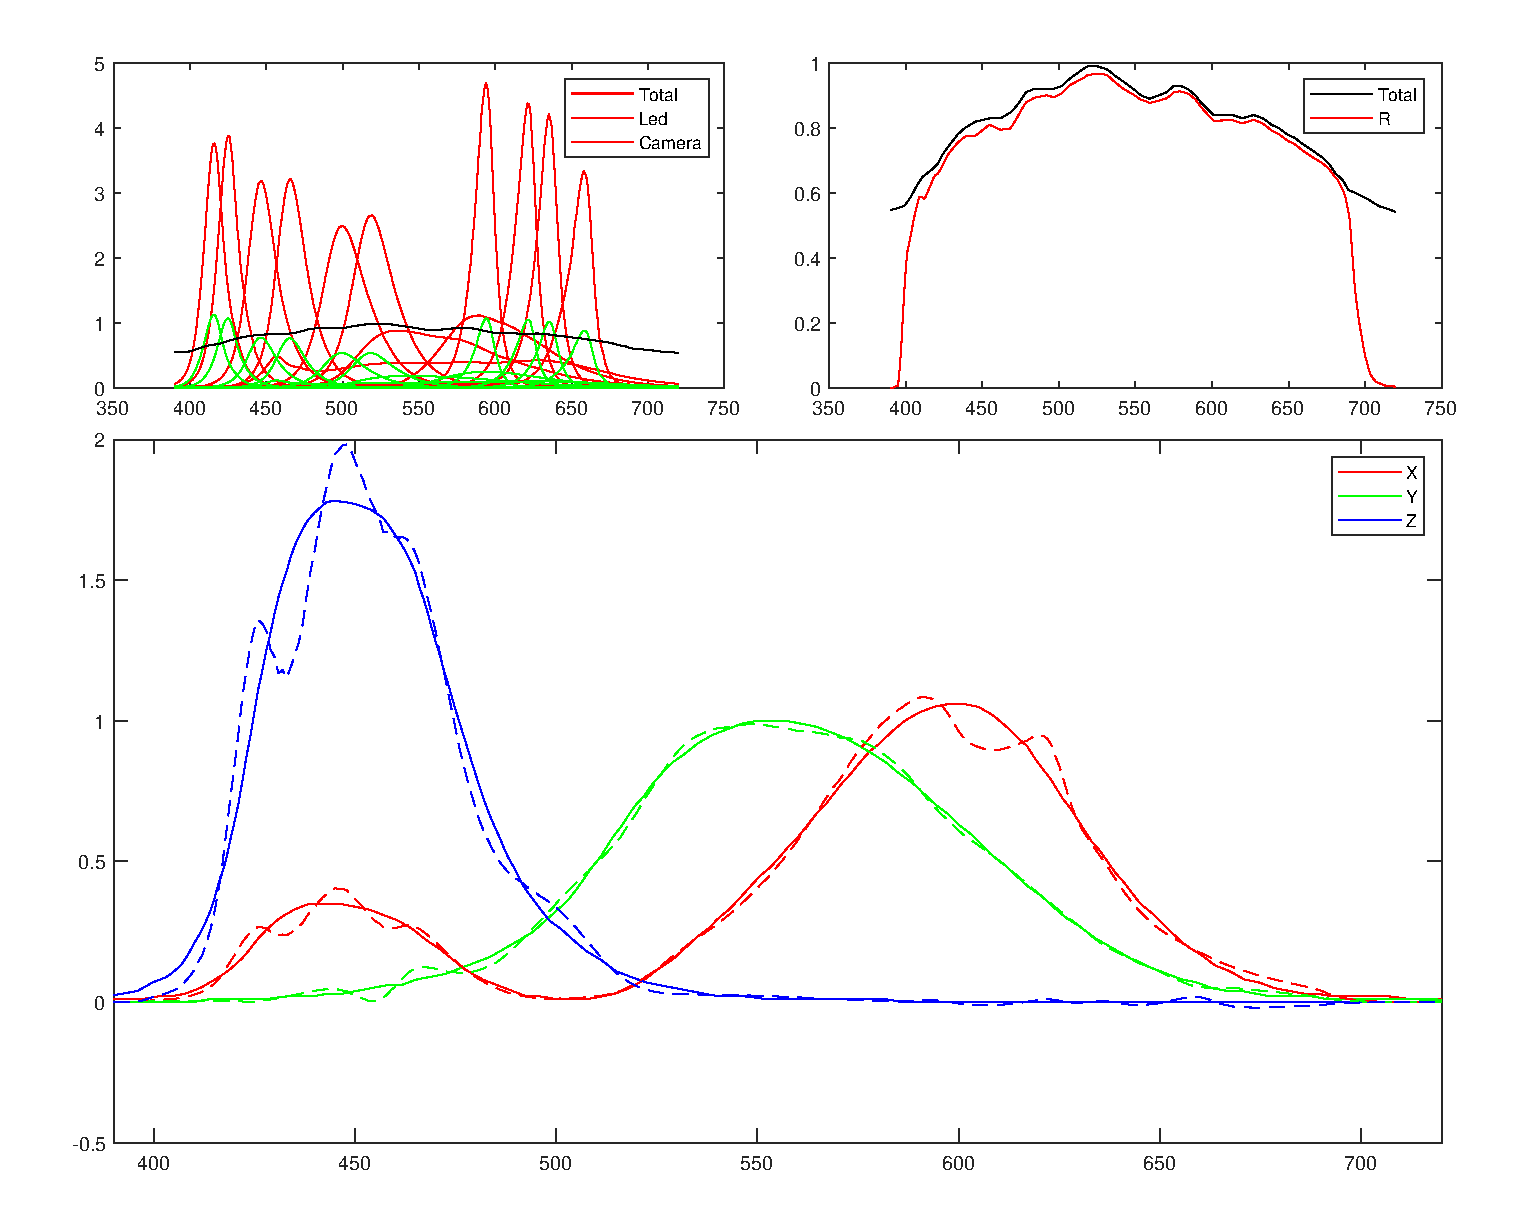
\includegraphics[width=1\linewidth]{chart.eps}
		\caption{Multispectral to RGB charts (top left: specular distribution of light sources, top right: specular response of camera, bottom: reference XYZ response combined with theoretical spectral response of merged images taken in combination with each led)} 
		\label{Figure 1}
	\end{center} 
\end{figure} 
\newpage
\bibliography{TextureScanner.bib}
\vspace*{\fill}
\textsuperscript{\textcopyright} 2023 Niklas Hauber, All rights reserved.
\end{document}